\part{Método}

\chapter[Método]{Método}\label{Capitulo4}

\section{Processo de Software}

O processo de desenvolvimento de software é algo complexo devido a variáveis que podem ter diferentes perspectivas de resultados.
Por isso é preciso definir soluções que atendam o objetivo do cliente de forma concisa. 
Aplicamos a metodologia ágil do Scrum, que nos ajudou na agilidade do processo de software, definindo as ações em cada atividade, a saber: (i) levantamento de requisitos, (ii) implementação do sistema e (iii) implantação do sistema.

Optamos por uma metodologia ágil, que é mais indicada para cenários como o nosso, equipe pequena e prazo curtos.
Com ela pudemos aplicar um fluxo de forma mais ágil, levantamos os requisitos, identificamos os problemas e definimos as soluções.
Em seguida, documentamos essas soluções através dos casos de uso e iniciamos a implementação, adotando as tecnologias e arquitetura com as quais temos mais experiência.

\section{Levantamento de Requisitos}

Através do levantamento de requisitos determinamos o problema.
Essa identificação foi feita através de reuniões com o setor de compras do IFG câmpus Formosa, em que resumimos os seguintes tópicos:

\begin{itemize}
    \item Descentralização das informações necessárias.
    \item Problemas de comunicação entre os interessados.  
    \item Problemas de comunicação na fase interna.  
    \item Problema com a solicitação de pedidos.
\end{itemize}

Com esses pontos notamos que o maior problema da fase interna era a comunicação. 
Com base nesses tópicos continuamos o levantamento de requisitos e montamos soluções hipotéticas usando casos de uso, que depois foram validados com o cliente.

\begin{itemize}
    \item O caso de uso~\ref{CASO001} mantém os dados sobre  materiais, serviços, itens e licitações atualizados.
    
    \item O caso de uso~\ref{CASO002} permite ao usuário solicitar a inclusão de itens e suas quantidades em uma licitação.

    \item O caso de uso~\ref{CASO003} permite que o usuário avalie o pedido de participação na licitação.
    
    \item O caso de uso~\ref{CASO004} permite que o usuário veja a resposta do pedido de participação na licitação.

\end{itemize}

%Portanto nossa solução é centralizar as informações necessárias para a participação de outros campus na licitação e melhorar a comunicação entre eles.

\section{Implementação do Sistema}

Desenvolvemos o sistema usando um \textit{framework} chamado JHipster na versão 4.13.2 que gera o esqueleto da aplicação, deixando pronta todo um \textit{front-end} básico, o \textit{back-end}, a comunicação entre entre eles e a integração com o banco de dados.

%E com isso conseguimos agilizar o processo desenvolvimento da aplicação web pois o ambiente de desenvolvimento foi montado de forma rápida e 

Utilizamos a API de compras governamentais para buscar as informações necessárias sobre itens, materiais, serviços e licitação.
Estes dados são então salvos no nosso banco de dados.

A implementação da aplicação foi baseada em uma \textit{stack} (pilha) de programas.
Para o desenvolvimento da estrutura lógica do sistema e integração com o banco de dados utilizamos JPA na versão 2.1 e o Hibernate na versão 5.2.12. Utilizamos \textit{Spring boot} na versão 1.5.9 para auxiliar no desenvolvimento criando uma API com arquitetura REST para a comunicação com o front-end.
Os dados foram persistidos no SGBD MySQL na versão 5.7 conforme o modelo de dados mostrado na~\ref{Figura007}.

\begin{sidewaysfigure}[ht]
	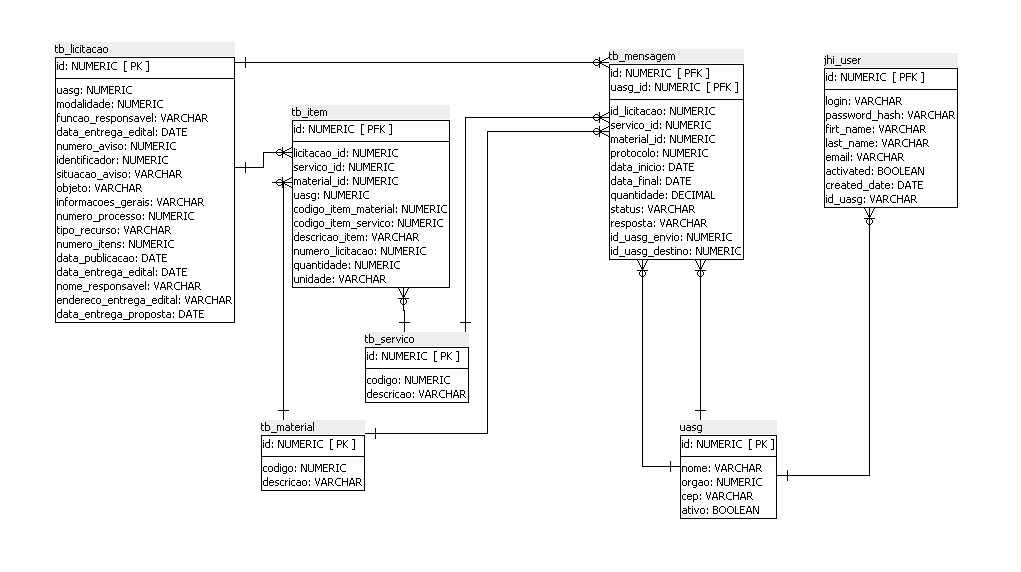
\includegraphics[width=0.95\textwidth]{figuras/bdAtualizado.png}
	\caption{Modelo de dados do projeto.}
	\label{Figura007}
\end{sidewaysfigure}

\begin{landscape}
\begin{table}[ht]
	\centering
\begin{tabular}{|l|l|l|l|}
	\hline
	Nome da Tabela & Nome da Coluna            & Comentário                                                             & Tipo do Dado \\ \hline
	tb\_licitacao  & id                        & Identificador da tabela.                                               & NUMERIC      \\ \hline
	tb\_licitacao  & uasg                      & Codigo da Unidades Administrativas de Serviços Gerais.                 & NUMERIC      \\ \hline
	tb\_licitacao  & modalidade                & Código da modalidade da licitação.                                     & NUMERIC      \\ \hline
	tb\_licitacao  & funcao\_responsavel       & Função do responsavel da licitação.                                    & VARCHAR      \\ \hline
	tb\_licitacao  & data\_entrega\_edital     & Data da entrega do edital.                                             & DATE         \\ \hline
	tb\_licitacao  & numero\_aviso             & Número do Aviso da Licitação por Registro de Preço.                    & NUMERIC      \\ \hline
	tb\_licitacao  & identificador             & Identificador da licitação associada.                                  & NUMERIC      \\ \hline
	tb\_licitacao  & situacao\_aviso           & Situação do aviso.                                                     & VARCHAR      \\ \hline
	tb\_licitacao  & objeto                    & Objeto da Licitação.                                                   & VARCHAR      \\ \hline
	tb\_licitacao  & informacoes\_gerais       & Informações Gerais.                                                    & VARCHAR      \\ \hline
	tb\_licitacao  & numero\_processo          & Número do Processo.                                                    & NUMERIC      \\ \hline
	tb\_licitacao  & tipo\_recurso             & Tipo do Recurso.                                                       & VARCHAR      \\ \hline
	tb\_licitacao  & numero\_itens             & Número de Itens.                                                       & NUMERIC      \\ \hline
	tb\_licitacao  & data\_publicacao          & Data da publicação da licitação.                                       & DATE         \\ \hline
	tb\_licitacao  & data\_entrega\_edital     & Data de Entrega do Edital.                                             & DATE         \\ \hline
	tb\_licitacao  & nome\_responsavel         & Nome do responsável pela licitação.                                    & VARCHAR      \\ \hline
	tb\_licitacao  & endereco\_entrega\_edital & Endereço de Entrega do Edital.                                         & VARCHAR      \\ \hline
	tb\_licitacao  & data\_entrega\_proposta   & Data de entrega da proposta.                                           & DATE         \\ \hline
	tb\_item       & id                        & Identificador da tabela.                                               & NUMERIC      \\ \hline
	tb\_item       & licitacao\_id             & Identificador da tabela tb\_licitacao.                                 & NUMERIC      \\ \hline
	tb\_item       & servico\_id               & Identificador da tabela tb\_servico.                                   & NUMERIC      \\ \hline
	tb\_item       & material\_id              & Identificador da tabela tb\_material.                                  & NUMERIC      \\ \hline
	tb\_item       & uasg                      & Codigo da Unidades Administrativas de Serviços Gerais.                 & NUMERIC      \\ \hline
	tb\_item       & codigo\_item\_material    & Código do Material.                                                    & NUMERIC      \\ \hline
	tb\_item       & codigo\_item\_servico     & Código do Serviço.                                                     & NUMERIC      \\ \hline
	tb\_item       & descricao\_item           & Descrição do item.                                                     & VARCHAR      \\ \hline
	tb\_item       & numero\_licitacao         & Identificador da licitação associada.                                  & NUMERIC      \\ \hline
	tb\_item       & quantidade                & Quantidade de itens de licitação.                                      & NUMERIC      \\ \hline
	tb\_item       & unidade                   & Unidade.                                                               & VARCHAR      \\ \hline
	tb\_material   & id                        & Identificador da tabela.                                               & NUMERIC      \\ \hline
	tb\_material   & codigo                    & Código do material.                                                    & NUMERIC      \\ \hline
	tb\_material   & descricao                 & Descrição do material.                                                 & VARCHAR      \\ \hline
\end{tabular}

\end{table}
\end{landscape}

\begin{landscape}
	\begin{table}[ht]
		\centering
		\begin{tabular}{|l|l|l|l|}
				\hline
			Nome da Tabela & Nome da Coluna            & Comentário                                                             & Tipo do Dado \\ \hline
			tb\_servico    & id                        & Identificador da tabela.                                               & NUMERIC      \\ \hline
			tb\_servico    & codigo                    & Código do serviço.                                                     & NUMERIC      \\ \hline
			tb\_servico    & descricao                 & Descrição do serviço.                                                  & VARCHAR      \\ \hline
			tb\_mensagem   & id                        & Identificador da tabela.                                               & NUMERIC      \\ \hline
			tb\_mensagem   & uasg\_id                  & Identificador da tabela tb\_uasg.                                      & NUMERIC      \\ \hline
			tb\_mensagem   & id\_licitacao             & Identificador da tabela tb\_licitacao.                                 & NUMERIC      \\ \hline
			tb\_mensagem   & servico\_id               & Identificador da tabela tb\_servico.                                   & NUMERIC      \\ \hline
			tb\_mensagem   & material\_id              & Identificador da tabela tb\_material.                                  & NUMERIC      \\ \hline
			tb\_mensagem   & protocolo                 & Protocolo gerado pelo sistema para o usuario identificar a requisição. & NUMERIC      \\ \hline
			tb\_mensagem   & data\_inicio              & Data da criação da requisição.                                         & DATE         \\ \hline
			tb\_mensagem   & data\_final               & Data da resposta da requisição.                                        & DATE         \\ \hline
			tb\_mensagem   & quantidade                & Quantidade de itens requisitados.                                      & DECIMAL      \\ \hline
			tb\_mensagem   & status                    & Status da mensagem.                                                    & VARCHAR      \\ \hline
			tb\_mensagem   & resposta                  & Resposta da Mensagem.                                                  & VARCHAR      \\ \hline
			tb\_mensagem   & id\_uasg\_envio           & Identificador da tabela uasg que solicitou a requisição.               & NUMERIC      \\ \hline
			tb\_mensagem   & id\_uasg\_destino         & Identificador da tabela uasg de destino requisição.                    & NUMERIC      \\ \hline
			tb\_uasg       & id                        & Identificador da tabela.                                               & NUMERIC      \\ \hline
			tb\_uasg       & nome                      & Nome da uasg.                                                          & VARCHAR      \\ \hline
			tb\_uasg       & orgao                     & Orgão que a uasg pertence.                                             & NUMERIC      \\ \hline
			tb\_uasg       & cep                       & CEP da Uasg                                                            & VARCHAR      \\ \hline
			tb\_uasg       & ativo                     & situação uasg                                                          & BOOLEAN      \\ \hline
			jhi\_user      & id                        & Identificador da tabela.                                               & NUMERIC      \\ \hline
			jhi\_user      & login                     & Login do usuario.                                                      & VARCHAR      \\ \hline
			jhi\_user      & password\_hash            & Senha do usuario criptografada.                                        & VARCHAR      \\ \hline
			jhi\_user      & firt\_name                & Primeiro nome do usuario.                                              & VARCHAR      \\ \hline
			jhi\_user      & last\_name                & Ultimo nome do usuario.                                                & VARCHAR      \\ \hline
			jhi\_user      & email                     & Email do usuario.                                                      & VARCHAR      \\ \hline
			jhi\_user      & activated                 & Usuario ativo                                                          & BOOLEAN      \\ \hline
			jhi\_user      & created\_date             & Data da criação do usuario.                                            & DATE         \\ \hline
			jhi\_user      & id\_uasg                  & Uasg do usuario.                                                       & VARCHAR      \\ \hline
		\end{tabular}
		
	\end{table}
\end{landscape}

Como o sistema é Web, o front-end foi criado utilizando  HTML e CSS, auxiliados por \textit{scripts} JavaScript para dar dinamismo na forma de apresentação de dados.
O AngularJS na versão 1.x auxiliou no desenvolvimento estabelecendo a comunicação entre o \textit{front-end} e o \textit{back-end}, além da criação das rotas do sistema.
Na estilização da tela usamos componentes \textit{on demand} do \textit{framework} O Bootstrap.

A arquitetura do nosso sistema é apresentada da~\prototipo{Figura005}.
O \textit{front-end} realiza chamadas de método para o \textit{back-end}, o qual as processa, se for o caso busca os dados no banco de dados, e retorna-os para o front-end.
O \textit{front-end} depende do \textit{back-end} apenas para os dados, mantendo-se visível ao usuário, independente da ação.

\begin{sidewaysfigure}[ht]
    \centering
    \includegraphics[width=0.95\textwidth]{figuras/figura005.png}
    \caption{Arquitetura do projeto.}
    \label{Figura005}
\end{sidewaysfigure}

\section{Implantação do Sistema}

A implantação do sistema ainda não ocorreu.
A implantação é agora dependente do cliente, o qual deverá proporcionar aos desenvolvedores uma agenda para a a validação das soluções implementadas.